\subsection{implementación en PCB}

\lipsum[3]\\

\begin{figure}[h]
    \centering
    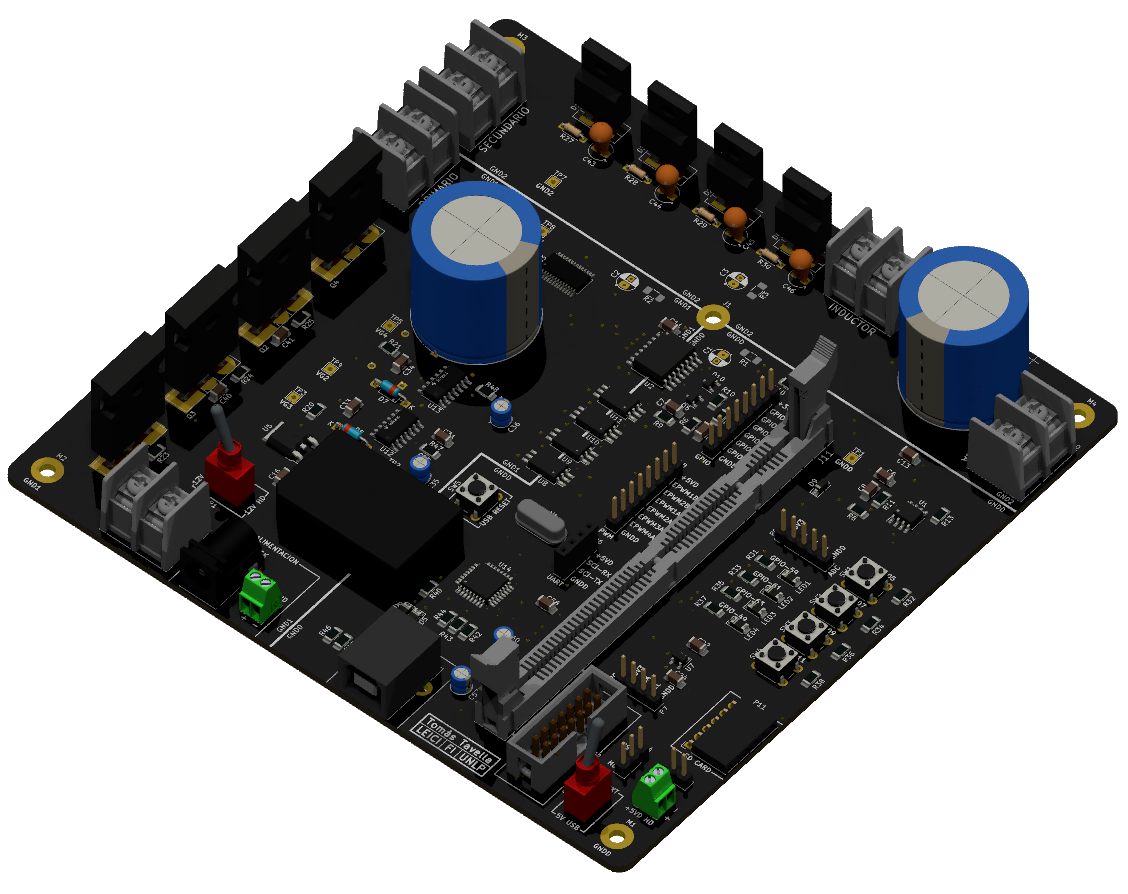
\includegraphics[scale=0.32]{Imagenes/PCB 3D Raytracing.png}
    \caption{Modelo tridimensional de la implementación en PCB de la plataforma con todos sus componentes, vista desde la parte superior.}
    \label{fig:PCB_3D}
\end{figure}

\lipsum[4]\\

\newpage\afterpage{\blankpage}

\begin{figure}[H]
    \centering
    \subfigure{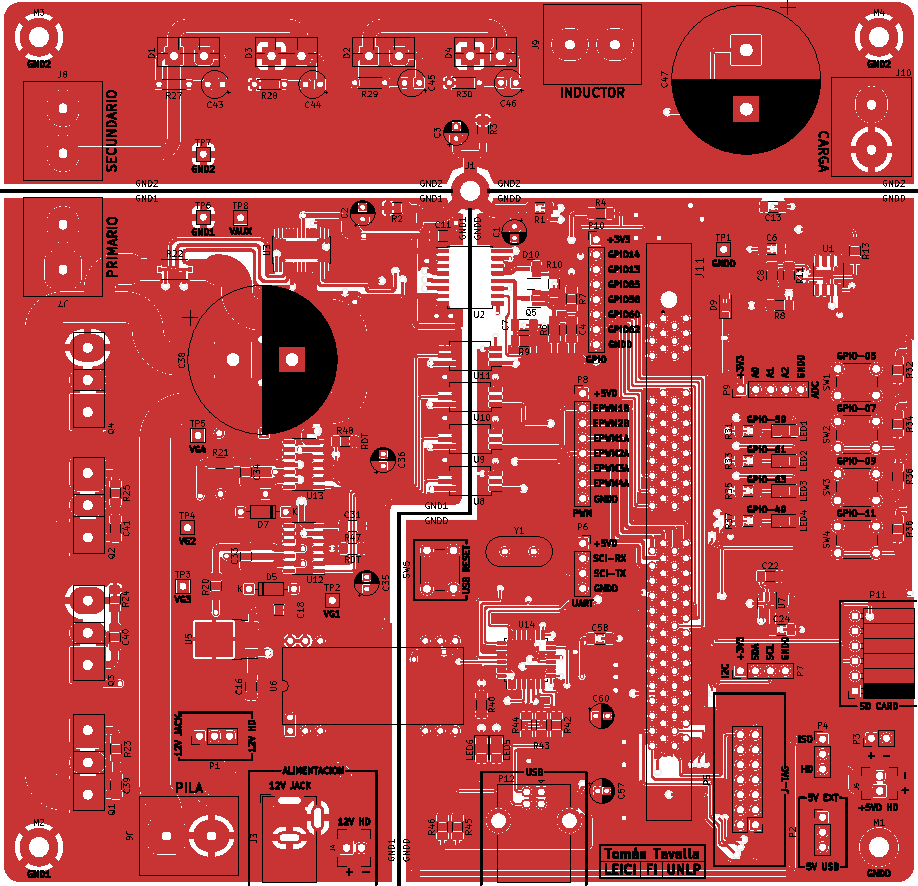
\includegraphics[scale=0.8]{Imagenes/PCB Front Layer.pdf}}\\
    \subfigure{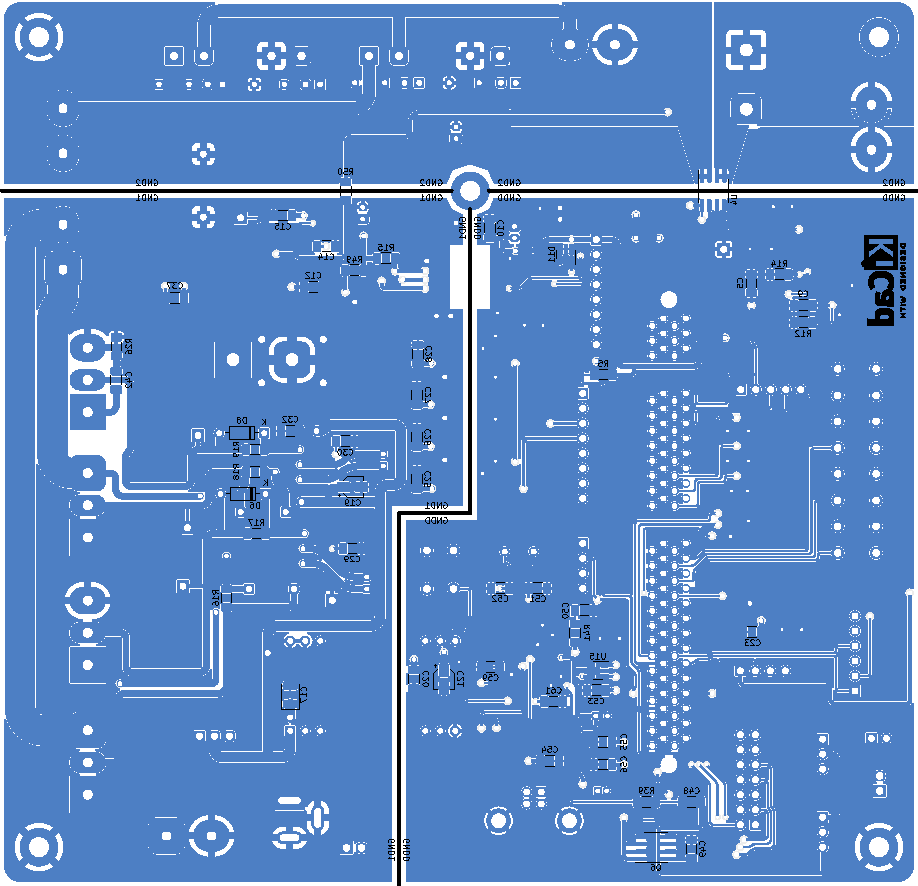
\includegraphics[scale=0.8]{Imagenes/PCB Back Layer.pdf}}%
    \caption{Diagrama de ambas capas de cobre de la PCB. La imagen superior corresponde a la capa frontal y la inferior a la capa trasera.}
    \label{fig:PCB_cobre}
\end{figure}